\chapter{طراحی و پیاده‌سازی}
در این بخش، طراحی و پیاده‌سازی بخش‌های مختلف سخت‌افزاری و نرم‌افزاری شرح داده خواهد شد.
<<<<<<< HEAD
\section{مقدمه}به صورت کلی، طراحی پروژه در تصویر \ref{arc1} است. همانطور که در تصویر مشخص شده است، میزبان اطلاعات را از پایگاه‌داده دریافت کرده و به هر دو برنامه سمت مشتری می‌فرستد. برنامه‌ای که جمع‌آورندگان سفارش از آن استفاده می‌کنند به صورت وب و در تلفن همراه هوشمند نمایش داده می‌شود. همچنین برنامه‌ای که برای تعیین کردن جایگاه محصولات استفاده می‌شود، بر روی نمایشگر لمسی که به یک بورد رزبری‌پای مدل \lr{3A} وصل شده است نمایش داده می‌شود.
=======
\section{مقدمه}به صورت کلی، طراحی پروژه در تصویر \ref{arc1} است. همانطور که در تصویر مشخص شده است، میزبان اطلاعات را از پایگاه‌داده دریافت کرده و به هر دو برنامه سمت مشتری می‌فرستد. برنامه‌ای که جمع‌آورندگان سفارش از آن استفاده می‌کنند به صورت وب و در تلفن همراه هوشند نمایش داده می‌شود. همچنین برنامه‌ای که برای تعیین کردن جایگاه محصولات استفاده می‌شود، بر روی نمایشگر لمسی که به یک بورد رزبری‌پای مدل \lr{3A} وصل شده است نمایش داده می‌شود.
>>>>>>> 0b914906bc0a1f3ca7b01ffa78967759bf4780dc

در این پروژه، رزبری‌پای صرفا وظیفه نمایش اطلاعات به کاربر و همچنین دریافت اطلاعات از کاربر و ارسال آن به میزبان اطلاعات است. کلیه برنامه‌های سمت کاربر، برنامه‌های سمت میزبان و همچنین پایگاه‌داده بر روی یک ماشین مجازی\LTRfootnote{\lr{Virtual Machine}} اجرا شده‌اند و تمامی فرآیندها بر روی منابع ماشین مجازی انجام می‌شوند. به همین دلیل رزبری‌پای کمترین فشار محاسباتی را متحمل می‌شود.
برای راه‌اندازی اولیه پروژه، ماشین مجازی با واحد محاسباتی تک‌هسته‌ای\LTRfootnote{\lr{1 Core CPU}}، 2 گیگابایت ظرفیت حافظه\LTRfootnote{\lr{Memory}} و همچنین 50 گیگابایت ظرفیت حافظه سخت\LTRfootnote{\lr{Hard Disk}} درنظر گرفته شده است.
\begin{figure}[t!]
    \centering
    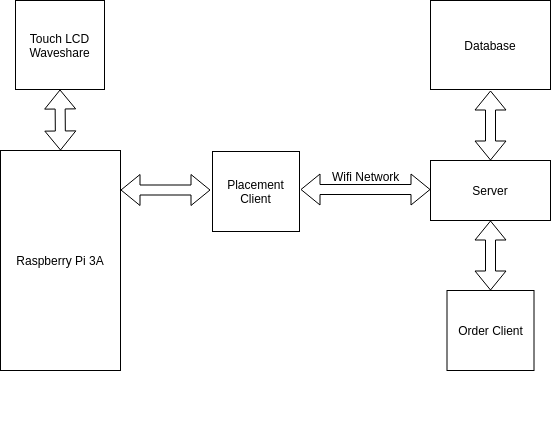
\includegraphics[scale=0.75]{figures/pro.png}
    \caption{معماری کلی پروژه}
    \label{arc1}
\end{figure}

در قسمت‌های بعد به تفصیل، طراحی و پیاده‌سازی هر کدام از این عناصر توضیح داده خواهد شد.

\section{نمایشگر لمسی}
در این قسمت به راه‌اندازی نمایشگر لمسی بر روی رزبری‌پای پرداخته خواهد شد.

\subsection{نحوه قرارگیری بر روی پین‌های \lr{GPIO}}
همانطور که در تصویر\ref{spi} مشخص است، این نمایشگر باید بر روی اولین پین‌های \lr{GPIO} رزبری‌پای قرار گیرد تا از طریق رابط سریال پیرامونی\LTRfootnote{\lr{Serial Peripheral Interface}} ارتباط برقرار شود.
\begin{figure}[t!]
    \centering
    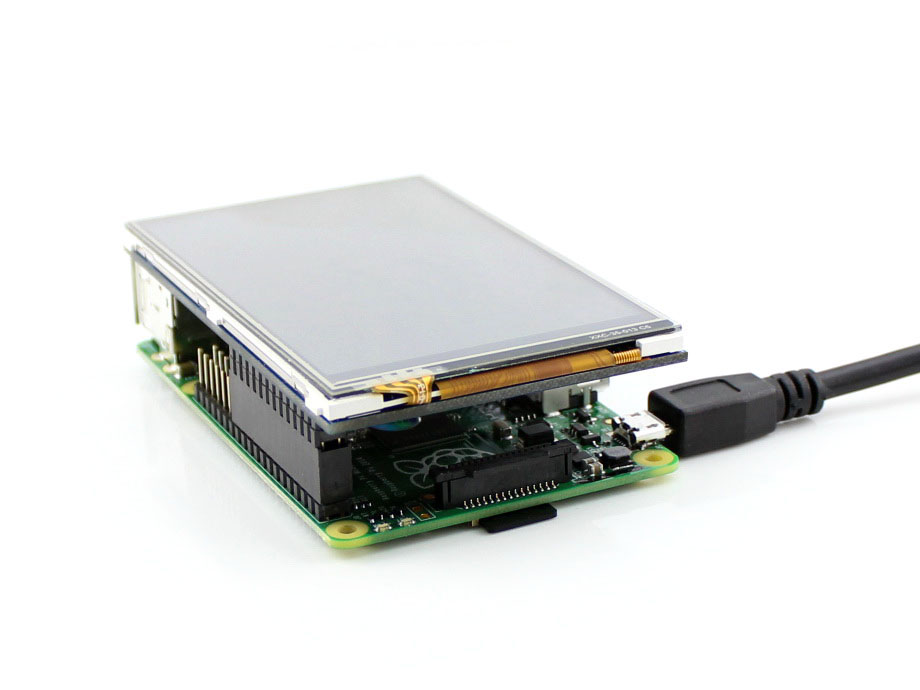
\includegraphics[scale=0.5]{figures/spi.jpg}
    \caption{قرارگیری نمایشگر لمسی بر روی رزبری‌پای }
    \label{spi}
\end{figure}

\subsection{راه‌اندازی نمایشگر بر روی رزبری‌پای}
پس از قرار دادن نمایشگر در جای مناسب، بورد را روشن کرده و با استفاده از آدرس  قرارداد اینترنتی\LTRfootnote{\lr{IP Address}} و نام‌کاربری، از طریق پوسته امن\LTRfootnote{\lr{SSH}} ارتباط برقرار شود.
یک راه برای پیدا کردن آدرس بورد، وصل کردن بورد به یک نمایشگر به وسیله کابل رابط چندرسانه ای وضوح بالا و باز کردن پایانه\LTRfootnote{\lr{Terminal}} و اجرای دستور زیر است:
\begin{latin}
    \begin{lstlisting}
        hostname -I
    \end{lstlisting}
\end{latin}

حال بر روی کامپیوتر مبدا، دستور پوسته امن به صورت زیر اجرا شود:
\begin{latin}
    \begin{lstlisting}
        ssh user@ip_address
    \end{lstlisting}
\end{latin}
توجه شود که \lr{user} نام کاربری موجود بر روی سیستم‌عامل رزبرین است. به طور پیش‌فرض مقدار آن \lr{pi} است. سپس رمز کاربر وارد شود.

حال باید تنظیماتی بر روی رزبری‌پای اعمال شود. برای این‌کار دستور زیر در پایانه اجرا شود:
\begin{latin}
    \begin{lstlisting}
        sudo raspi-config
    \end{lstlisting}
\end{latin}

در این قسمت \lr{Expand Filesystem} فعال شود. همچنین \lr{Boot Option} بر روی \lr{Desktop Autologin} قرار داده شود.

 پس از انجام تنظیمات اولیه، نمایشگر آماده نصب است. برای راه‌اندازی، ابتدا راه‌انداز نمایشگر با دستور زیر بارگیری شود:
\begin{latin}
    \begin{lstlisting}
        git clone https://github.com/waveshare/LCD-show.git
        cd LCD-show/
    \end{lstlisting}
\end{latin}

حال باید فایل صفرویکی \lr{LCD35-show} را اجرا کنیم. برای این کار در ابتدا‌ باید اجازه\LTRfootnote{\lr{permission}} اجرای فایل به وسیله دستور زیر داده شود:
\begin{latin}
    \begin{lstlisting}
        chmod +x LCD35-show
    \end{lstlisting}
\end{latin}
حال فایل زیر اجرا شود:

\begin{latin}
    \begin{lstlisting}
        ./LCD35-show
    \end{lstlisting}
\end{latin}
پس از انجام این مرحله، نمایشگر نصب شده است و با راه‌اندازی مجدد بورد، اطلاعات راه‌انداز بورد بر روی نمایشگر نشان داده خواهد شد. ولی قسمت لمسی نمایشگر باید تنظیم گردد تا محل تماس را بتواند به درستی تشخیص دهد. در مرحله بعد این تنظیم انجام می‌شود.

\subsection{تنظیم صفحه لمسی}
این نمایشگر با استفاده از برنامه‌ای به نام \lr{xinput\_calibrator} که به طور پیش‌فرض بر روی سیستم‌عامل رزبین نصب شده است، قابل تنظیم است. برای تنظیم نمایشگر، دستور زیر در پایانه وارد شود:

\begin{latin}
    \begin{lstlisting}
        sudo DISPLAY=:0.0 xinput_calibrator
    \end{lstlisting}
\end{latin}

همانطور که در تصویر \ref{calibrate} مشخص است، نقاطی بر روی نمایشگر نشان داده می‌شود که باید به ترتیب لمس شوند تا جایگاه دقیق بخش لمسی نمایشگر تشخیص داده شود.
\begin{figure}[t!]
    \centering
    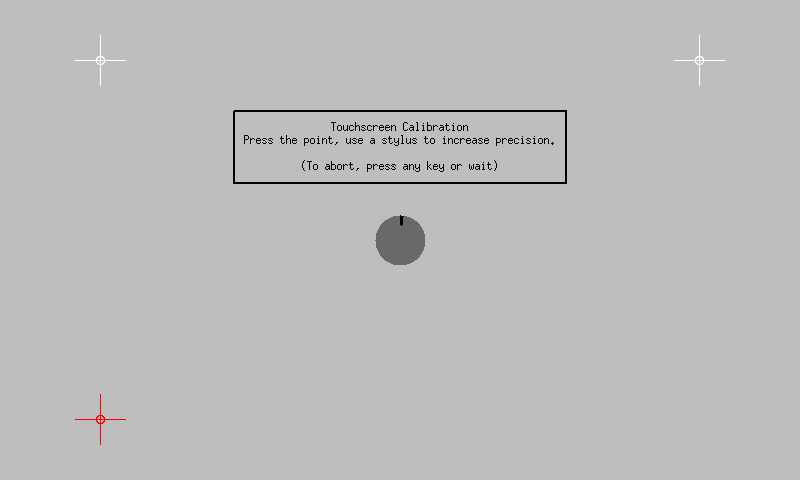
\includegraphics[scale=0.5]{figures/calibrate.png}
    \caption{تنظیم صفحه نمایش لمسی }
    \label{calibrate}
\end{figure}

پس از اتمام این مرحله خروجی مشابه زیر چاپ می‌شود:
\begin{latin}
    \begin{lstlisting}
        Doing dynamic recalibration:
        Setting new calibration data: 3919, 208, 236, 3913
    \end{lstlisting}
\end{latin}

به وسیله یک ویرایشگر، فایل \lr{99-calibration.conf} را ویرایش کرده و با اطلاعات بالا جایگزین شود. برای نمونه با استفاده از ویرایشگر \lr{VIM} ای فایل در آدرس زیر قابل ویرایش است:
\begin{latin}
    \begin{lstlisting}
        sudo vim /etc/X11/xorg.conf.d/99-calibration.conf
    \end{lstlisting}
\end{latin}

حال به وسیله دستور زیر، رزبری‌پای راه‌اندازی مجدد شود.
\begin{latin}
    \begin{lstlisting}
        sudo reboot
    \end{lstlisting}
\end{latin}


\section{طراحی و پیاده‌سازی پایگاه‌داده}
با توجه به نیازمندی‌های مطرح شده، پایگاه‌داده به صورت نمودار \ref{uml} طراحی شد.

\begin{figure}[t!]
    \centering
    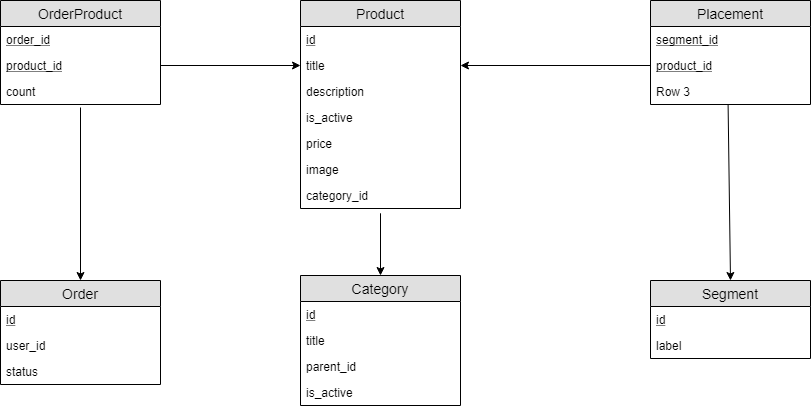
\includegraphics[scale=0.5]{figures/uml.png}
    \caption{طراحی پایگاه‌داده }
    \label{uml}
\end{figure}

\subsection{محصولات}
محصولات در جدول \lr{Product} با مشخصه‌های زیر طراحی شد:

\begin{itemize}
   	\item \textbf{\lr{id}}: شناسه محصول - کلید اصلی
   	\item \textbf{\lr{title}}: عنوان محصول 
	\item \textbf{\lr{description}}: توضیحات محصول
	\item \textbf{\lr{is\_active}}: فعال یا غیرفعال بودن محصول
	\item \textbf{\lr{price}}: قیمت محصول
	\item \textbf{\lr{image}}: تصویر محصول
	\item \textbf{\lr{category}}: کلید خارجی به جدول \lr{Category}
\end{itemize}

\subsection{سفارش‌ها}
سفارش‌ها در جدول \lr{Order} با مشخصه‌های زیر طراحی شد:
\begin{itemize}
   	\item \textbf{\lr{id}}: شناسه سفارش - کلید اصلی
   	\item \textbf{\lr{user\_id}}: شناسه مشتری 
	\item \textbf{\lr{status}}: وضعیت فعلی سفارش. وضعیت فعلی سفارش یا \lr{registered} است و یا \lr{picked}. اگر سفارشی ثبت شده باشد و محصولاتش جمع‌آوری نشده باشد، وضعیت \lr{registered} است و اگر محصولات جمع‌آوری شد، به \lr{picked} تغییر پیدا می‌کند.
\end{itemize}

\subsection{بخش‌ها}
بخش‌ها در جدول \lr{Segment} با مشخصه‌های زیر طراحی شد:
\begin{itemize}
   	\item \textbf{\lr{id}}: شناسه بخش - کلید اصلی
   	\item \textbf{\lr{label}}: برچسب بخش
\end{itemize}

\subsection{دسته‌بندی‌ها}
دسته‌بندی‌ها در جدول \lr{Category} با مشخصه‌های زیر طراحی شد:
\begin{itemize}
   	\item \textbf{\lr{id}}: شناسه دسته‌بندی - کلید اصلی
   	\item \textbf{\lr{title}}: عنوان دسته‌بندی
   	\item \textbf{\lr{parent\_id}}: پدر دسته فعلی
   	\item \textbf{\lr{is\_active}}: فعال یا غیرفعال بودن دسته
\end{itemize}

\subsection{جداول میانی}
برای ارتباط بین جداول معرفی شده، چندین جدول میانی طراحی گردید که ارتباط چند به چند بین این جداول را فراهم می‌کند.\\
جدول \lr{Placement} ارتباط بین محصولات و بخش‌های مختلف را نشان می‌دهد که دارای مشخصه‌های زیر است:
\begin{itemize}
   	\item \textbf{\lr{product\_id}}: شناسه محصول
   	\item \textbf{\lr{segment\_id}}: شناسه بخش
   	\item \textbf{\lr{count}}: تعداد
\end{itemize}
در این جدول هیچ سطری وجود ندارد که دارای شناسه محصول و شناسه بخش یکسان باشند.\\

جدول \lr{OrderProduct} ارتباط بین محصولات و سفارش‌های مختلف را نشان می‌دهد که دارای مشخصه‌های زیر است:
\begin{itemize}
   	\item \textbf{\lr{product\_id}}: شناسه محصول
   	\item \textbf{\lr{order\_id}}: شناسه سفارش
   	\item \textbf{\lr{count}}: تعداد
\end{itemize}
در این جدول هیچ سطری وجود ندارد که دارای شناسه محصول و شناسه سفارش یکسان باشند.\\

\section{رابط‌های برنامه‌نویسی نرم‌افزار}
همانطور که در قسمت معرفی تکنولوژی‌های مسئله توضیح داده شد، برای پیاده‌سازی رابط‌های برنامه نویسی نرم‌افزار پروژه از چهارچوب نرم‌افزاری \lr{Django Rest API}
استفاده شد. با توجه به نیازمندی‌های مسئله و برای برقراری ارتباط با برنامه سمت کاربر، رابط‌هایی که در ادامه معرفی می‌شوند طراحی و پیاده‌سازی شدند.

\subsection{دریافت محصولات فعال}
آدرس دریافت محصولات به این صورت تعریف شده است. روش\LTRfootnote{\lr{Method}} فراخوانی این آدرس از نوع \lr{GET} است.
\begin{latin}
    \begin{lstlisting}
        /api/products
        #output
        [
            {
                "id": 4,
                "title": "ThinkPad T480 - E",
                "description": "",
                "is_active": true,
                "price": 18800000,
                "image": "",
                "category": "%*\rl{لپتاپ}*)",
                "segments": [
                    "B-1"
                ]
            },
        ]

    \end{lstlisting}
\end{latin}

\subsection{لیست سفارش‌ها}
آدرس دریافت لیست سفارش‌ها به این صورت تعریف شده است. روش فراخوانی این آدرس از نوع \lr{GET} است.
\begin{latin}
    \begin{lstlisting}
        /api/orders
        #output
        [
            {
                "id": 4,
                "customer": "admin",
                "status": "picked",
                "products": [
                    {
                        "id": 4,
                        "title": "ThinkPad T480 - E",
                        "description": "",
                        "is_active": true,
                        "price": 18800000,
                        "image": "",
                        "category":  "%*\rl{لپتاپ}*)",
                        "segments": [
                            "B-1"
                        ]
                    },
                ],
                "created_at": "2019-08-26T09:56:29Z"
            }
        ]


    \end{lstlisting}
\end{latin}


\subsection{دریافت محصولات یک سفارش}
آدرس دریافت محصولات یک سفارش خاص به این صورت تعریف شده است. روش فراخوانی این آدرس از نوع \lr{GET} است.
\begin{latin}
    \begin{lstlisting}
        /api/order-products/1
        #output
        [
            {
                "id": 1,
                "customer": "admin",
                "status": "picked",
                "products": [
                    {
                        "id": 5,
                        "title": "MacBook Air MQD32 2017",
                        "description": "",
                        "is_active": true,
                        "price": 11175000,
                        "image": "",
                        "category": "%*\rl{لپتاپ}*)",
                        "segments": []
                    },
                ],
                "created_at": "2019-08-26T09:56:29Z"
            }
        ]
    \end{lstlisting}
\end{latin}


\subsection{لیست بخش‌ها}
آدرس دریافت بخش‌ها به این صورت تعریف شده است. روش فراخوانی این آدرس از نوع \lr{GET} است.
\begin{latin}
    \begin{lstlisting}
        /api/segments
        #output
        [
            {
                "id": 1,
                "label": "A-20"
            },
            {
                "id": 3,
                "label": "A-1"
            },
        ]
    \end{lstlisting}
\end{latin}


\subsection{ثبت جایگاه یک محصول}
آدرس ثبت جایگاه یک محصول در بخش مورد نظر به این صورت تعریف شده است. روش فراخوانی این آدرس از نوع \lr{POST} است.
بدنه درخواست\LTRfootnote{\lr{Request Body}} این رابط، لیستی از شناسه‌های محصولات است.
\begin{latin}
    \begin{lstlisting}
        /api/submit-segment/{segment_id}
    \end{lstlisting}
\end{latin}

\subsection{اطلاع اتمام جمع‌آوری محصولات سفارش}
آدرس اطلاع اتمام جمع‌آوری محصولات سفارش به این صورت تعریف شده است. روش فراخوانی این آدرس از نوع \lr{POST} است.
بدنه درخواست این رابط، لیستی از شناسه‌های محصولات است.
\begin{latin}
    \begin{lstlisting}
        /api/pick-order/{order_id}
    \end{lstlisting}
\end{latin}

\section{‌برنامه انتخاب محصولات بخش‌ها}
بر روی رزبری‌پای‌های موجود در هر بخش، مرورگری باز است که همواره یک صفحه برای انتخاب محصولات جدید آن بخش را نشان می‌دهد.

اما اولین بار که رزبری‌پای روشن می‌شود، آدرس زیر فراخوانی می‌شود:
\begin{latin}
    \begin{lstlisting}
        http://ip.com/segments
    \end{lstlisting}
\end{latin}
این صفحه که در تصویر \ref{segments} مشخص است، لیستی از بخش‌های موجود در انبار و یا فروشگاه‌ را نشان می‌دهد.
کاربر ابتدا باید بخش مورد نظر را انتخاب کرده تا به صفحه‌ای که به در تصویر \ref{segment} نمایش داده شده است، منتقل شود.
در این صفحه لیست تمامی محصولات موجود و فعال که مدیر برنامه اضافه کرده است نمایش داده می‌شود و کاربر پس از انتخاب محصولات موردنظر، دکمه تایید
را فشار می‌دهد تا اطلاعات محصولات جدید بخش، به میزبان فرستاده شود و در پایگاه‌داده ثبت گردد. همانطور که در تصاویر \ref{implement} و \ref{implement2} مشخص است، مسئولین چیدمان محصول در جایگاه‌ها می‌توانند با انتخاب محصولات از طریق نمایشگر و پس از لمس کردن گزینه تایید، جایگاه جدید محصولات را بروزرسانی کنند.
\begin{figure}[t!]
    \centering
    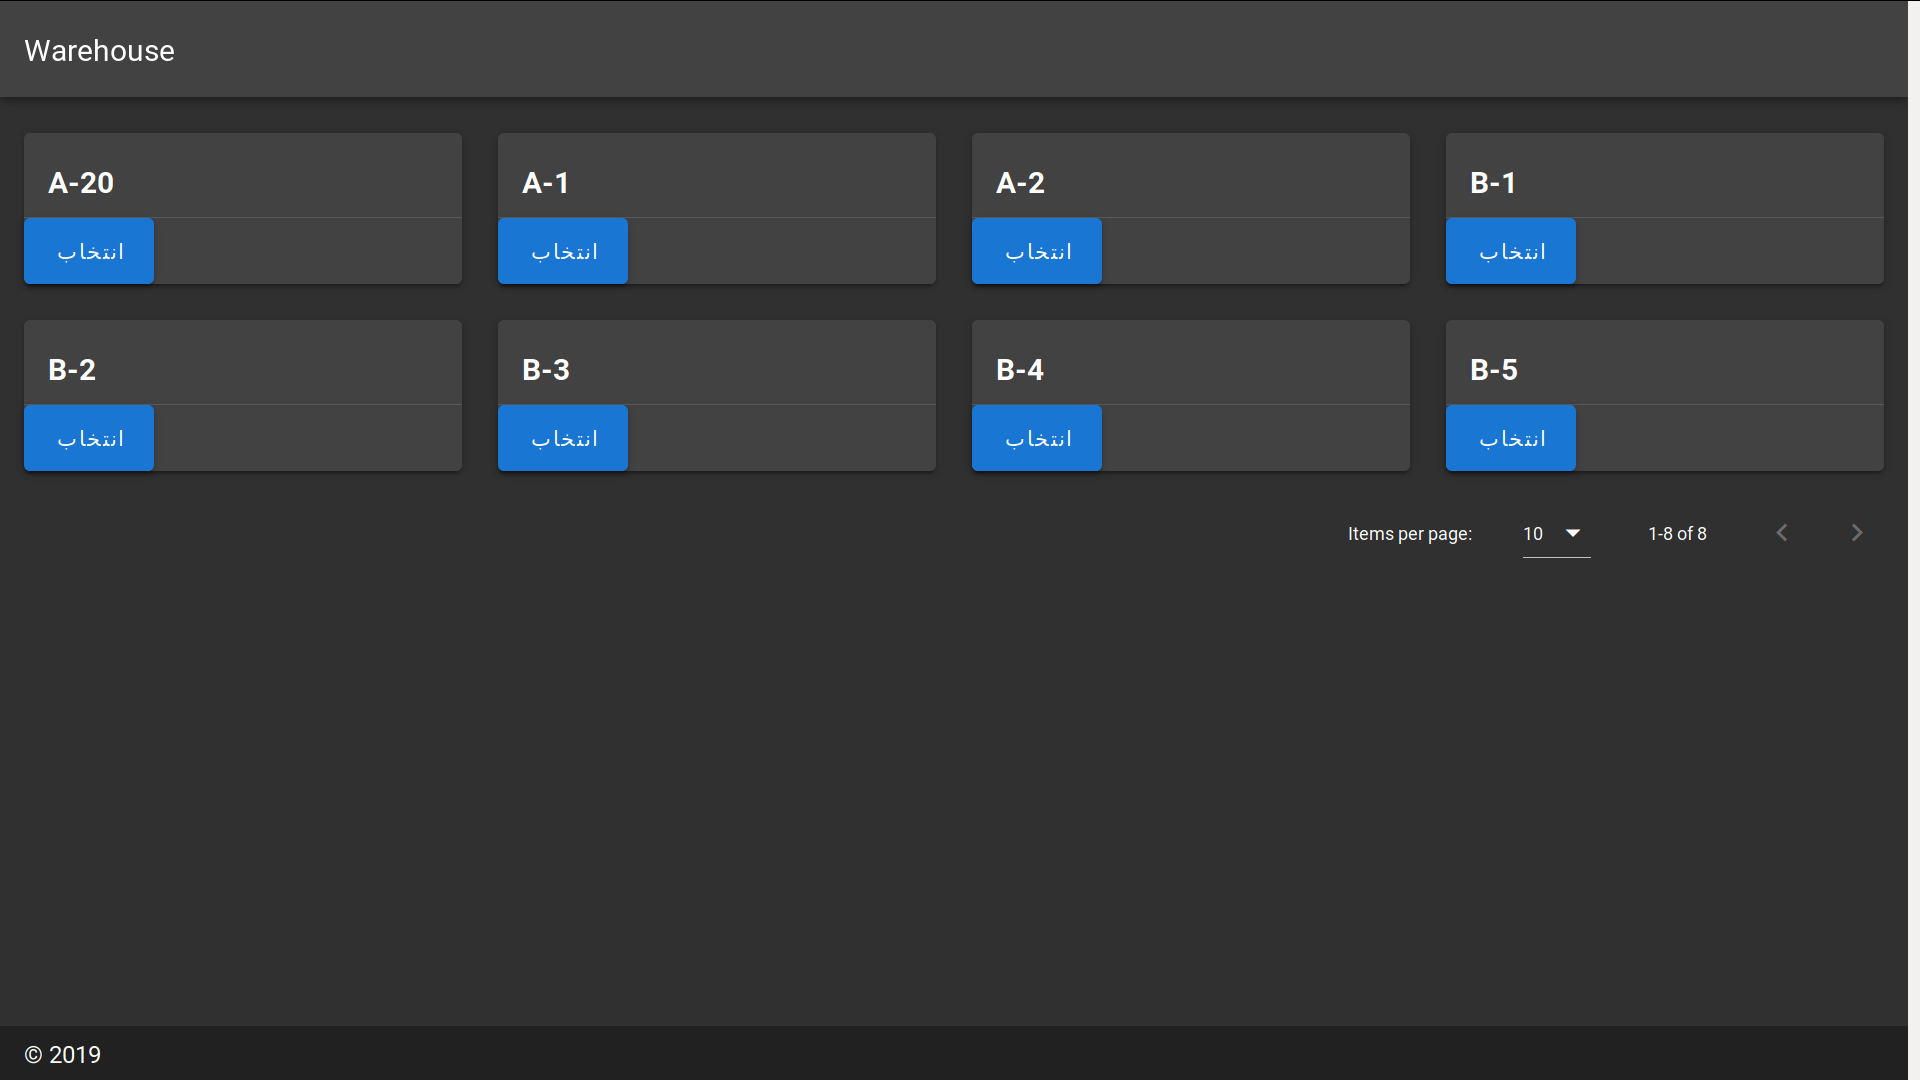
\includegraphics[scale=0.25]{figures/segments.png}
    \caption{نمایش بخش‌ها }
    \label{segments}
\end{figure}

\begin{figure}[t!]
    \centering
    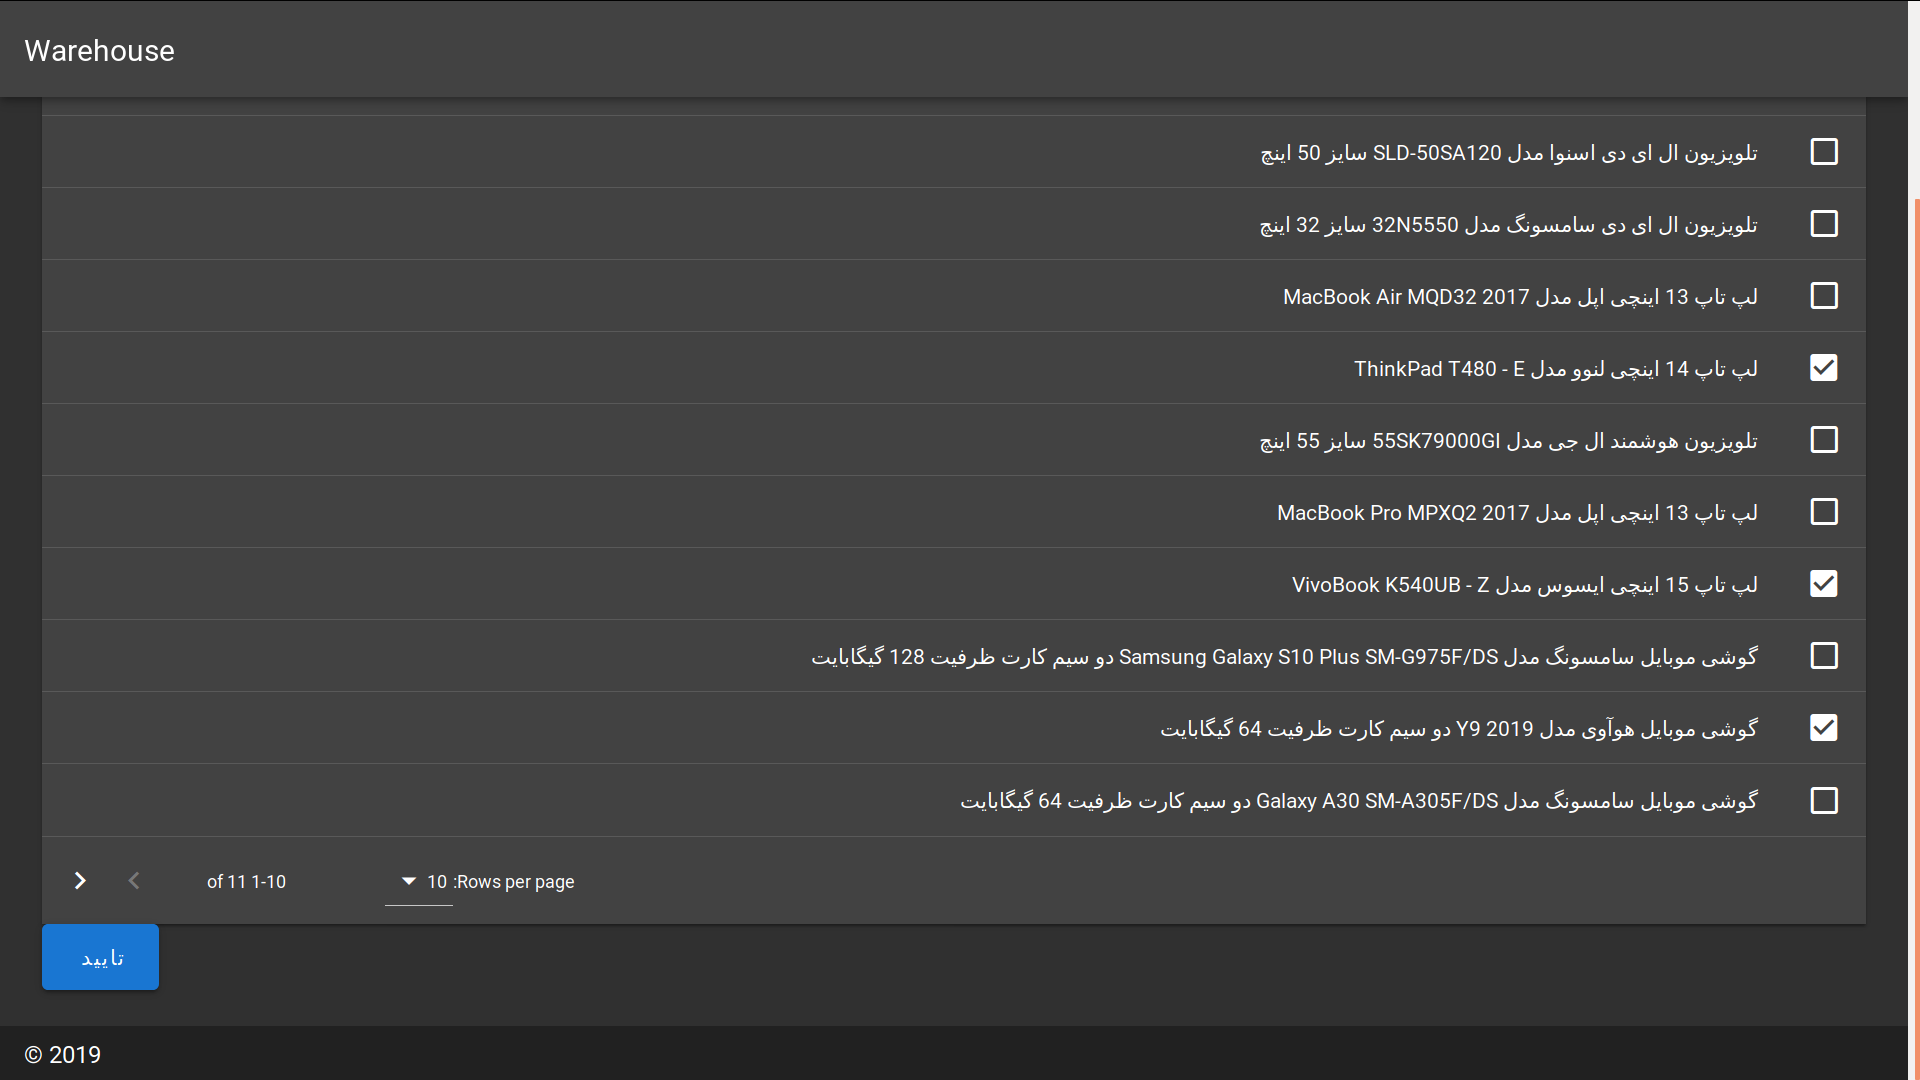
\includegraphics[scale=0.25]{figures/segment.png}
    \caption{نمایش محصولات جهت ثبت در بخش مورد نظر }
    \label{segment}
\end{figure}

\begin{figure}[t!]
    \centering
    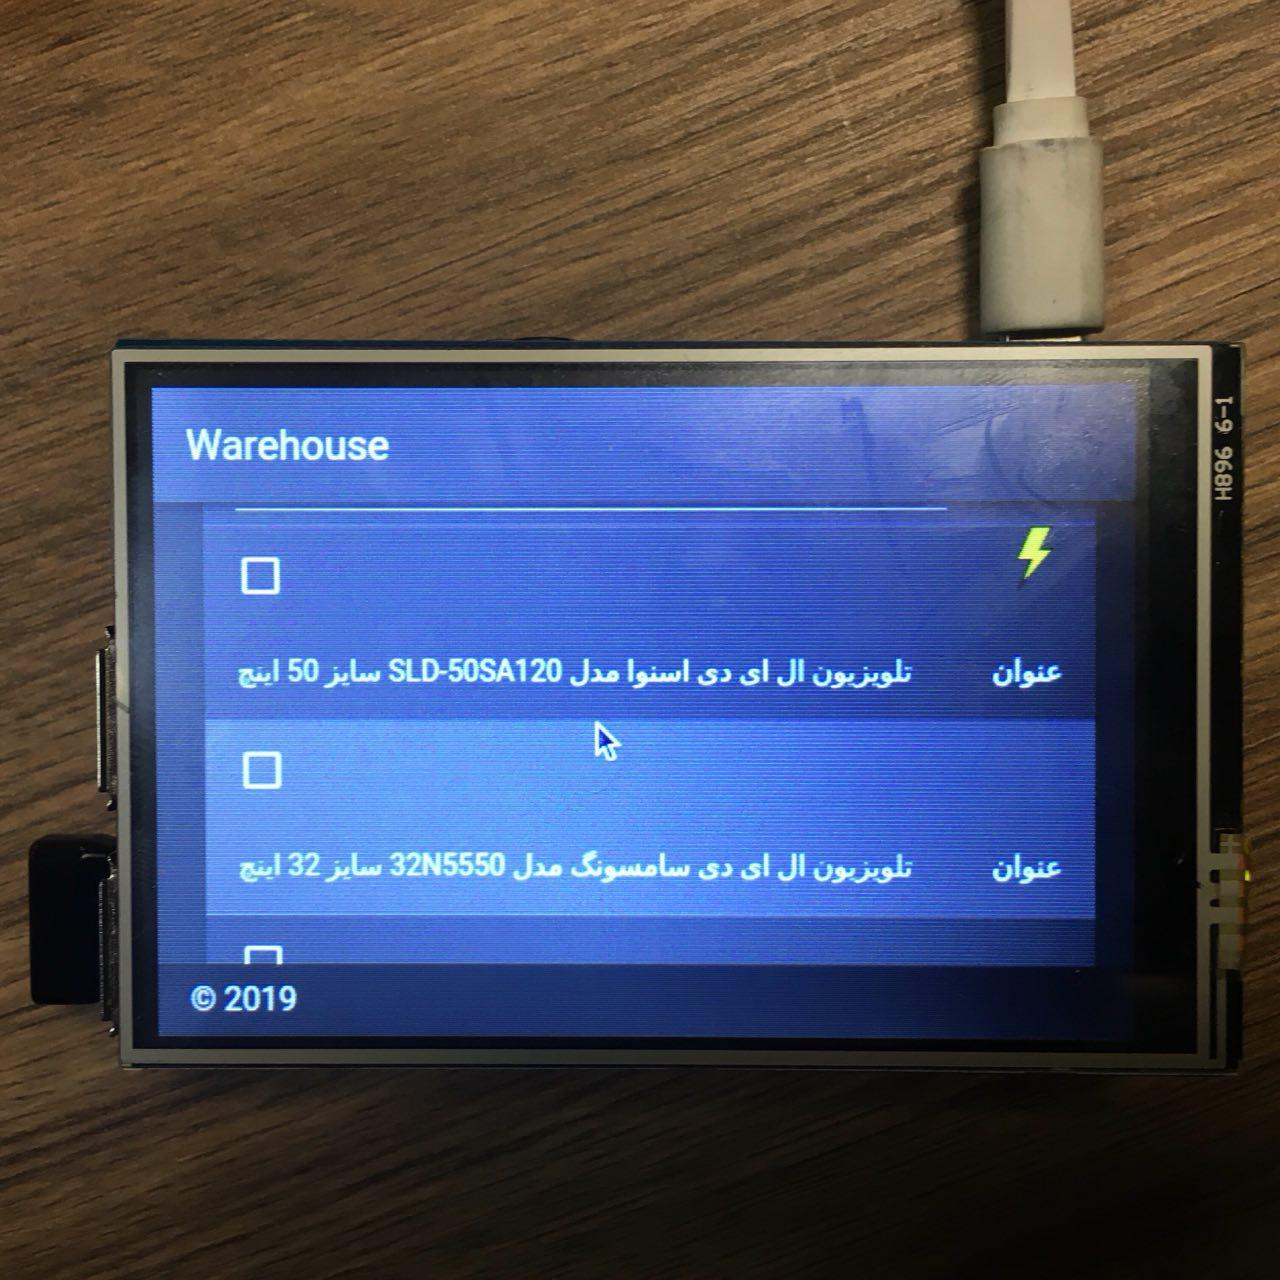
\includegraphics[scale=0.25]{figures/implement.jpg}
    \caption{نمایش لیست محصولات برنامه انتخاب محصولات بخش‌ها بر روی رزبری‌پای}
    \label{implement}
\end{figure}

\begin{figure}[t!]
    \centering
    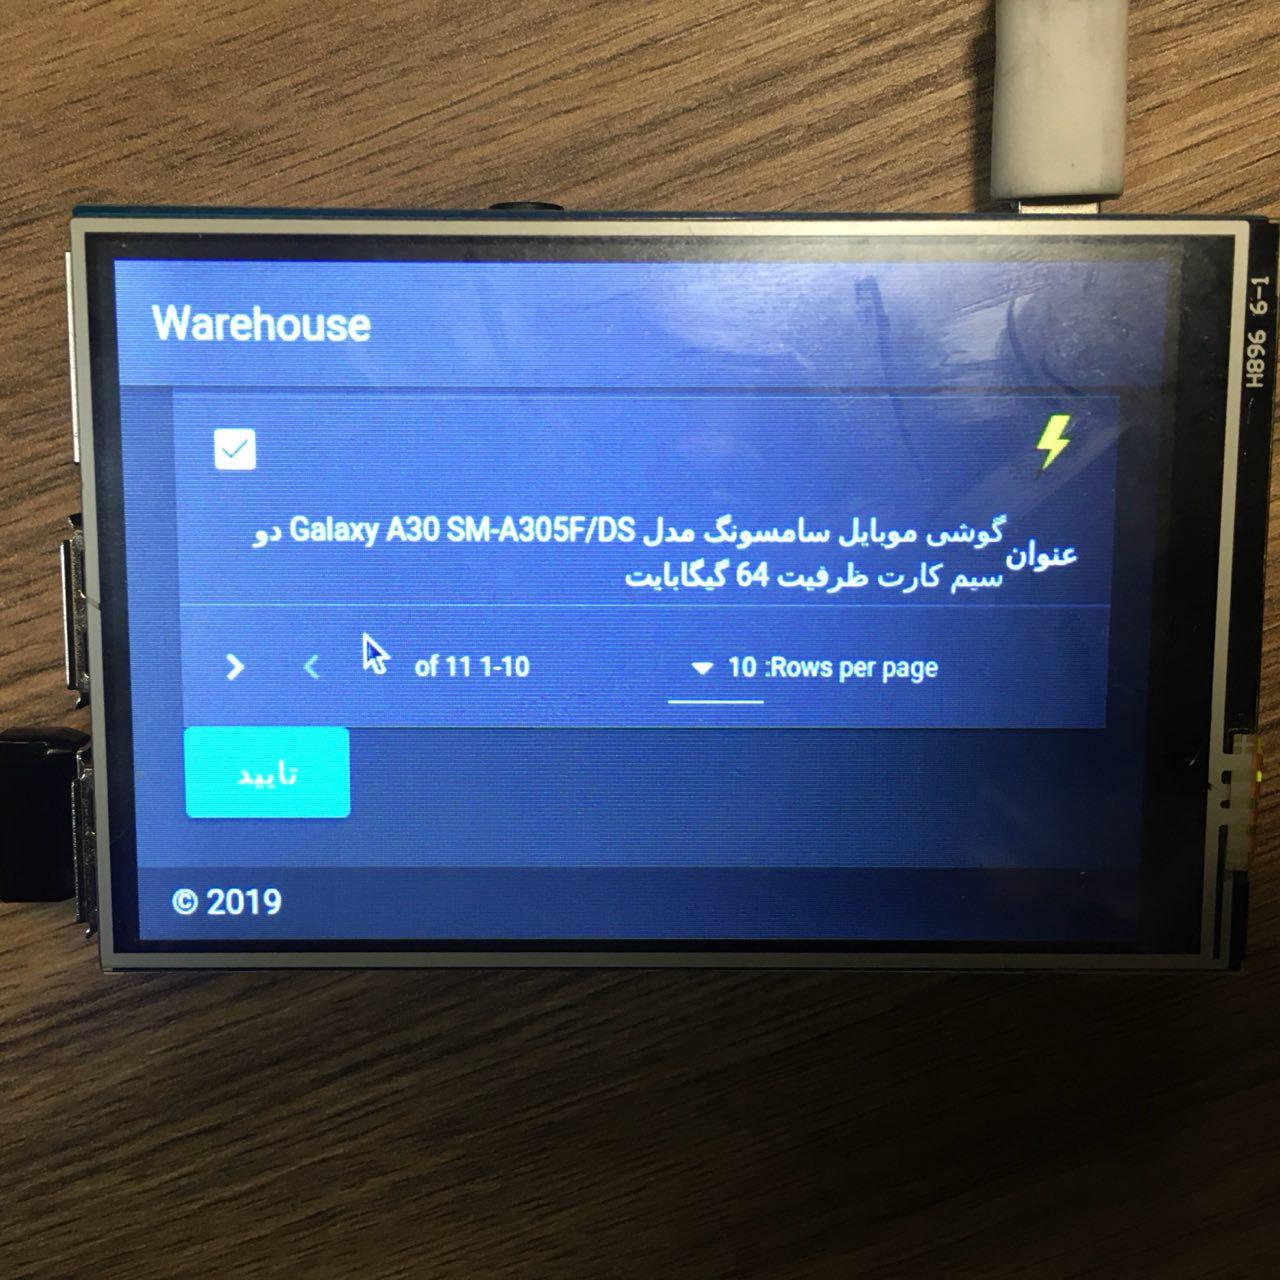
\includegraphics[scale=0.25]{figures/implement2.jpg}
    \caption{نمایش  گزینه تایید برنامه انتخاب محصولات بخش‌ها بر روی برزبری‌پای}
    \label{implement2}
\end{figure}

\section{برنامه جمع‌آوری محصول}
هنگامی که سفارشی ثبت می‌شود، وضعیت آن سفارش \lr{registered} است. مسئولان جمع‌آوری\LTRfootnote{\lr{picker}} سفارش، نیاز دارند لیستی از سفارش‌های ثبت
شده که هنوز جمع‌آوری نشده‌اند را ببینند. لیست این سفارش‌ها که در تصویر \ref{orders} مشخص است، در آدرس زیر موجود است:
\begin{latin}
    \begin{lstlisting}
        http://ip.com/orders
    \end{lstlisting}
\end{latin}
پس از انتخاب سفارش، مسئول جمع‌آوری لیستی از محصولات ثبت شده در سفارش را همراه با جایگاه آن‌ها مشاهده می‌کند. این صفحه در تصویر \ref{order} نمایش داده شده است.
هنگامی که مسئول جمع‌آوری محصولات سفارش را جمع‌آوری کرد، دکمه "جمع‌آوری شد" را فشار می‌دهد. این عمل تابعی را فراخوانی می‌کند
تا وضعیت سفارش را به \lr{picked} تغییر دهد.


\begin{figure}[t!]
    \centering
    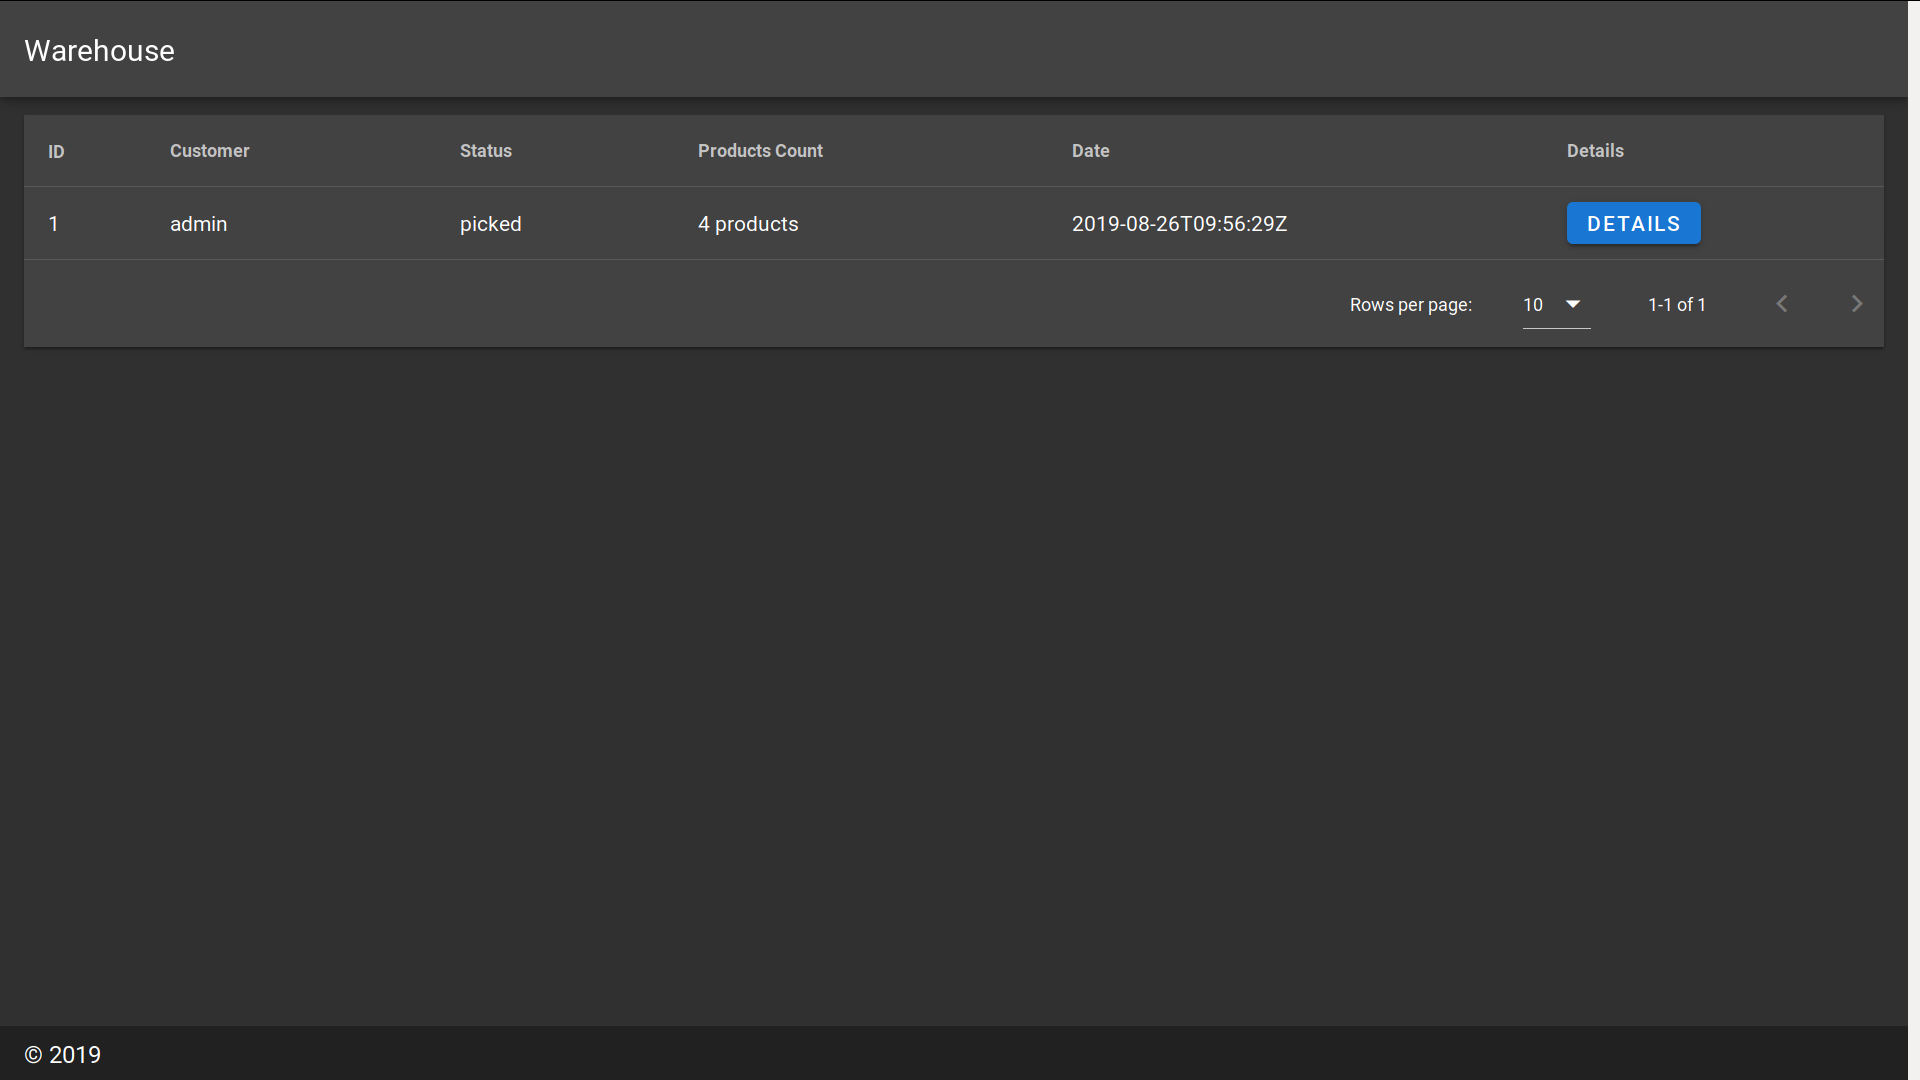
\includegraphics[scale=0.25]{figures/orders.png}
    \caption{لیست سفارش‌ها }
    \label{orders}
\end{figure}

\begin{figure}[t!]
    \centering
    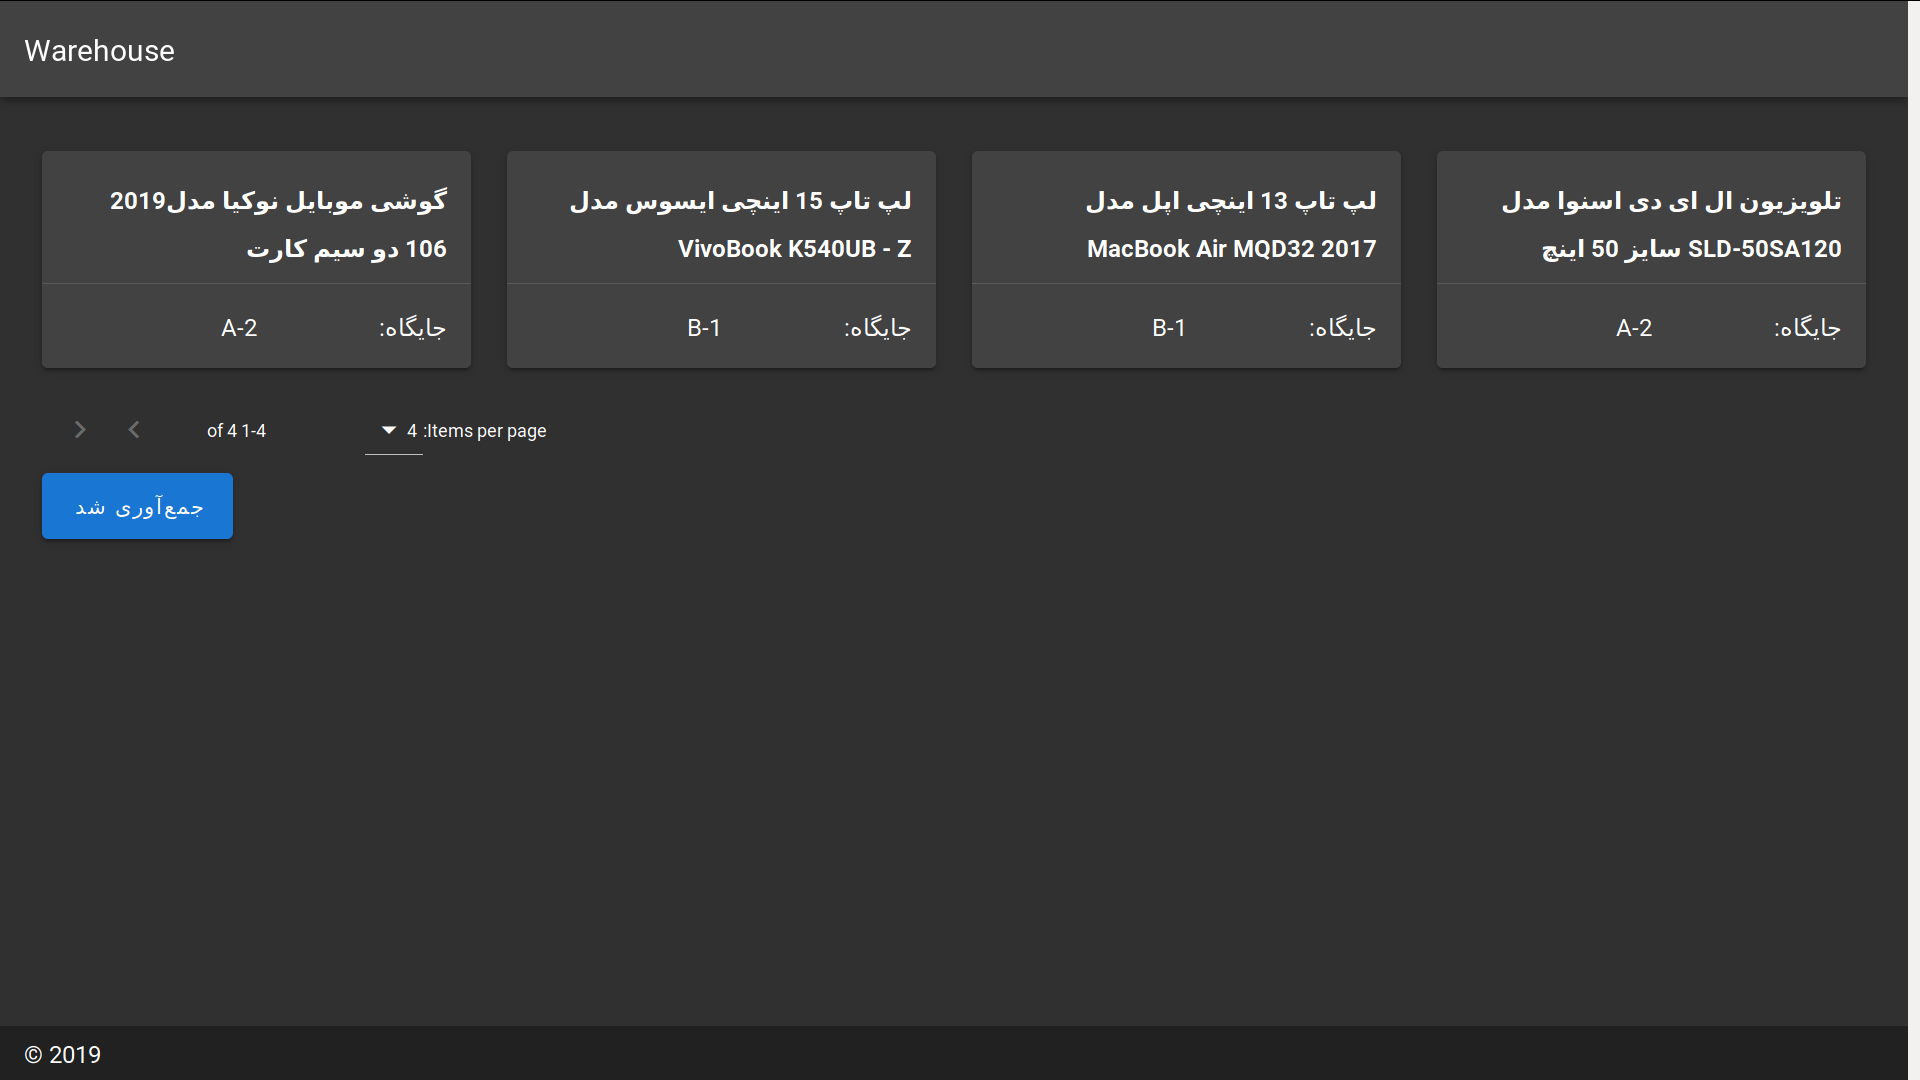
\includegraphics[scale=0.25]{figures/order.png}
    \caption{لیست محصولات سفارش }
    \label{order}
\end{figure}

\section{رابط کاربری مدیریت}
برای مدیریت عناصر موجود و همچنین با توجه به نیازمندی‌های مطرح شده، رابط کاربری برای مدیریت مجموعه طراحی و پیاده‌سازی شد.
در این قسمت امکاناتی فراهم شد که هرکدام به تفصیل توضیح داده خواهد شد. این قسمت توسط پیشوند \lr{admin} در دسترس است.

\subsection{احراز هویت و دسترسی}
برای پیاده‌سازی احراز هویت و همچنین دادن دسترسی به کاربران، از مدل کاربر-گروه\LTRfootnote{\lr{User-Group}} جنگو استفاده شده است.
در این سیستم دو ماهیت گروه و کاربر وجود دارد.
\begin{itemize}
   	\item \textbf{گروه}: مجموعه‌ای از افراد که برایشان دسترسی‌های یکسانی تعریف شده است.
   	\item \textbf{کاربر}: هر کاربر که توسط مدیر\LTRfootnote{\lr{Admin}} سایت ثبت‌نام می‌شود، می‌تواند به گروه‌های مختلف ملحق شود.
\end{itemize}
کاربران از طریق صفحه \ref{login} که از طریق آدرس زیر در دسترس است احراز هویت می‌شوند:
\begin{latin}
    \begin{lstlisting}
        http://ip.com/admin/login
    \end{lstlisting}
\end{latin}

\begin{figure}[t!]
    \centering
    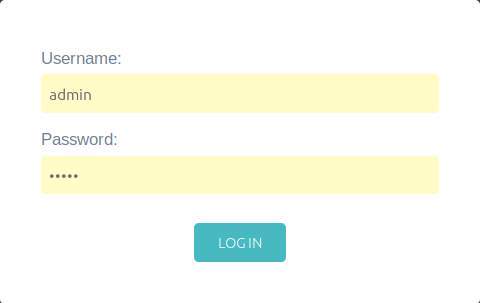
\includegraphics[scale=0.5]{figures/login.png}
    \caption{صفحه احراز هویت }
    \label{login}
\end{figure}



\subsection{ایجاد و ویرایش عناصر پایگاه‌داده}
برای راحتی مدیریت و کنترل محتوای پایگاه‌داده، صفحاتی ایجاد شد تا مدیر سایت توانایی ایجاد و ویرایش عناصر پایگاه داده، مانند محصولات، دسته‌بندی‌ها، بخش‌ها و سفارش‌ها را داشته باشد.

به طور کلی این بخش شامل موارد زیر است:
همچنین صفحات زیر برای مدیریت هرچه ساده‌تر پایگاه داده فراهم شد:
\begin{itemize}
   	\item اضافه کردن (تصویر \ref{new-product})، ویرایش (تصویر \ref{edit-product}) و یا حذف یک محصول
   	\item اضافه کردن، ویرایش و یا حذف یک دسته‌بندی
   	\item اضافه کردن، ویرایش و یا حذف یک بخش
   	\item مشاهده و ویرایش سفارش
\end{itemize}


\begin{figure}[t!]
    \centering
    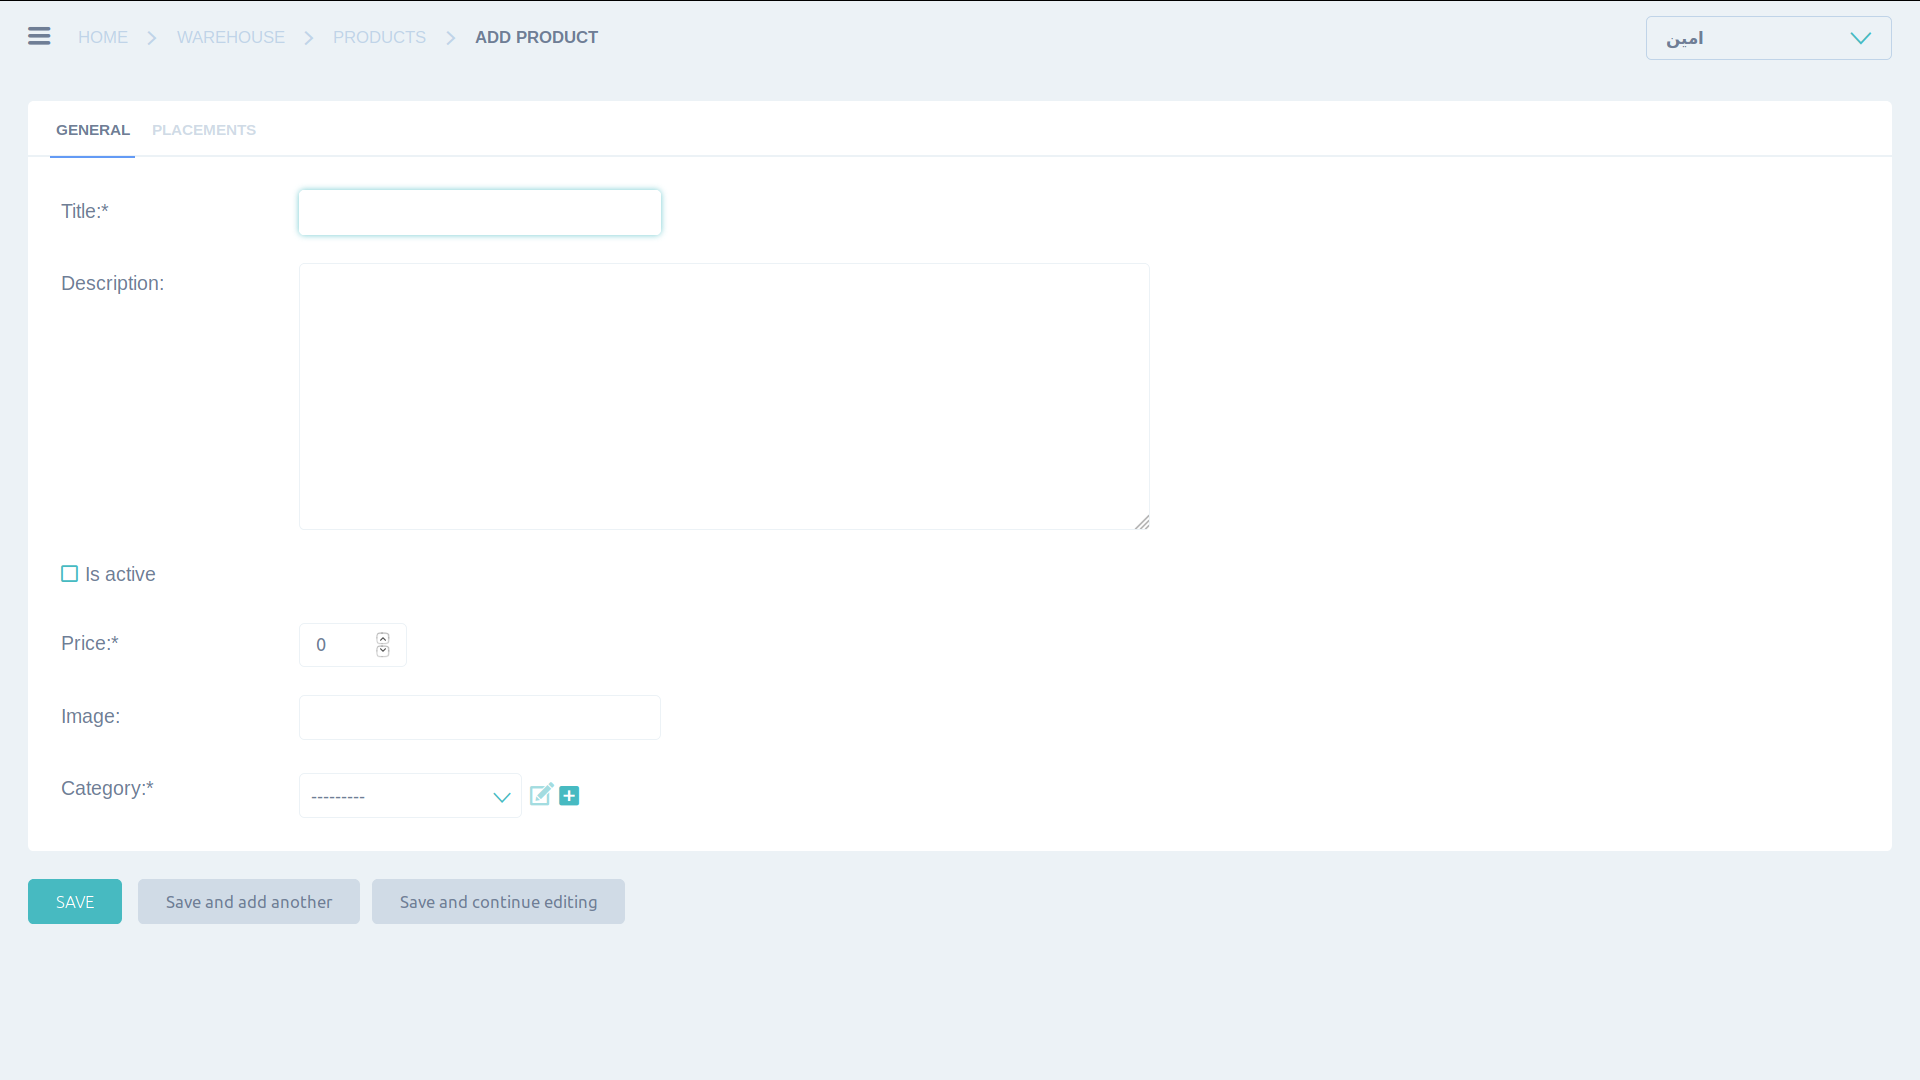
\includegraphics[scale=0.25]{figures/new-product.png}
    \caption{ایجاد محصول}
    \label{new-product}
\end{figure}

\begin{figure}[t!]
    \centering
    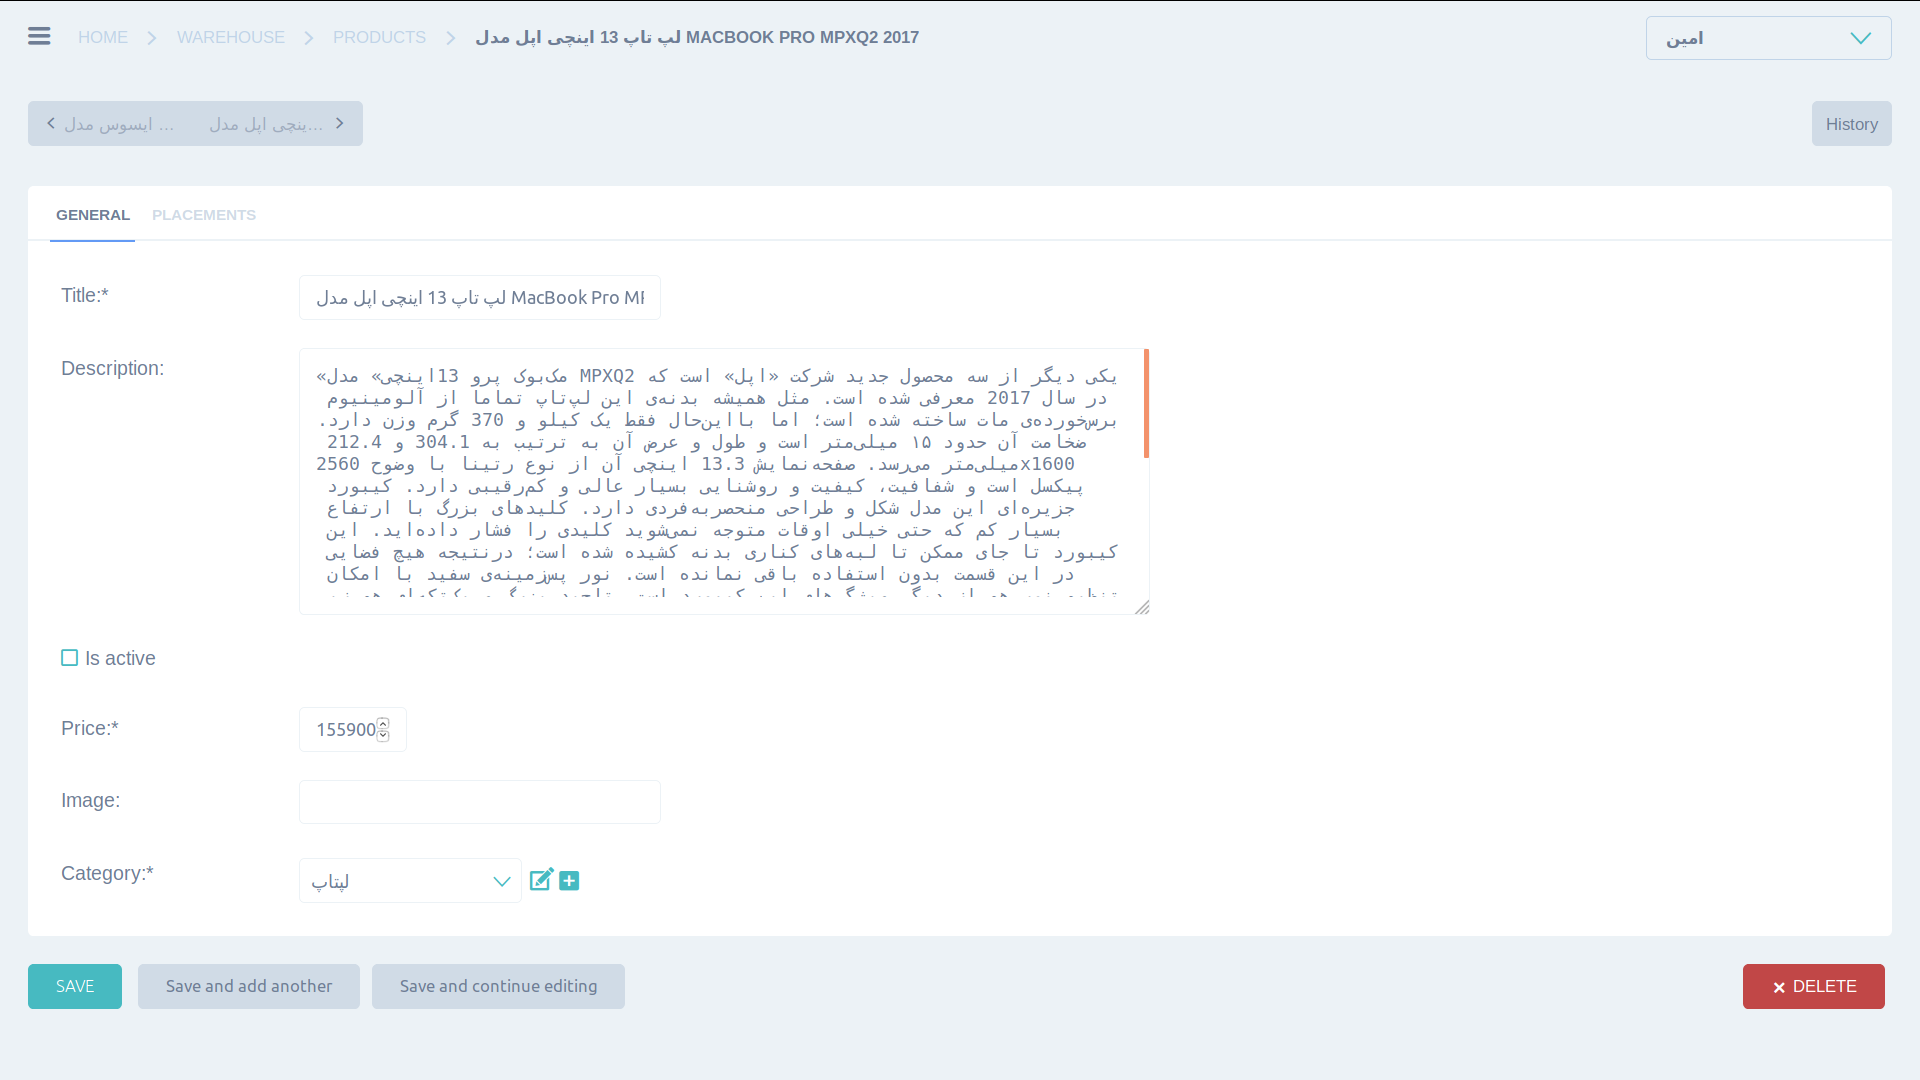
\includegraphics[scale=0.25]{figures/edit-product.png}
    \caption{ویرایش محصول}
    \label{edit-product}
\end{figure}


\section{نتیجه‌گیری}
در این پروژه برنامه‌های جمع‌آوری محصولات سفارش، تعیین جایگاه محصولات و همچنین رابط مدیریت پیاده‌سازی شد. برنامه جمع‌آوری محصول با استفاده از \lr{Nuxt.js} و همچنین \lr{Django}، داده‌های پایگاه‌داده را بروزرسانی می‌کند. همچنین برنامه تعیین جایگاه محصولات در بخش‌های مختلف، با استفاده از مرورگر نصب شده بر روی رزبری‌پای  به همراه نمایشگر لمسی نصب شده روی آن،  مورد استفاده قرارمی‌گیرد. با استفاده از \lr{Django}، رابط کاربری مدیریت نیز پیاده‌سازی شد.
